\section{Implementation and Runtime}
In this section we discuss our extensions to 
the MapReduce programming model and shows the major changes to runtime to 
support \myds
to support pipelining between Map and Reduce (Section 3.2). 
We describe how our design supports
piplelining (Section 3.3), and discuss the buffer design (Section 3.4). 
Our focus here is on Producer-Consumer model; 
We defer performance results to Section 5.



\subsection{Execution flow}
\begin{figure}[!h!t]  
    \centering
    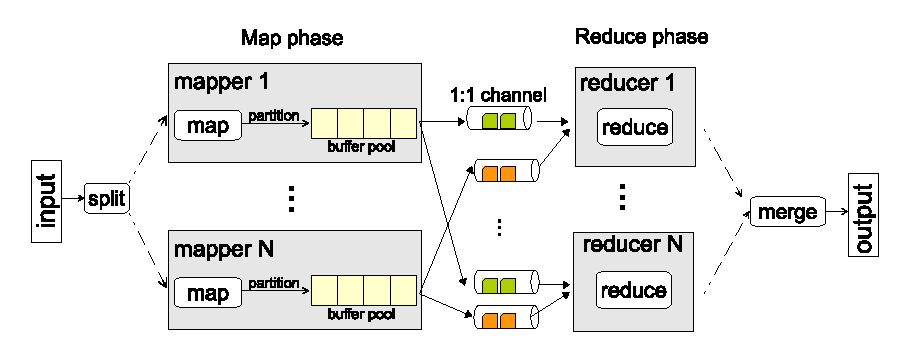
\includegraphics[width=0.5\textwidth]{eps/dmr_workflow.eps}
    \caption{The workflow of DMR}
    \label{fig:dmr:workflow}
\end{figure}

%不同与Phoenix,DMR将任务队列静态的划分给每个map worker,这样做的好处是,可以避免多个map worker对对任务队列操作从而产生锁的开销。
\myds's implementation of MapReduce closely resembles Phoenix’s. 
There is a single master managing a number of slaves worker. 
Figure\ref{fig:dmr:workflow} illustrates the workflow of \myds,
including three main phases: map, reduce, and merge. 
At the beginning, a split function divides the input
data as a task and push the task into a taskQueue. 
On multi-core CPUs, a worker is handled by one thread, 
which is a \myth thread in \myds.
%A worker usually needs to process multiple input elements. 
%Thus the map function is applied to the input elements one by one. 
%Such an operation of applying the map function for an input element is 
%called a map operation. 
%Each map operation produces intermediate key-value pairs. 
%Then a partition function is applied to these key-value pairs. 
%Then in the reduce phase, each reduce operation
%applies the reduce function to a set of intermediate pairs
%with the same key. 
Likely in cluster, the worker in Map phase pull a task from the queue, 
and apply the map function for the tasks.
Each map worker produces intermediate key-value pairs and insert them into a local buffer.
Then worker in Reduce phase will invoke reduce function to aggregates a set of intermediate pairs with the same key.  
Finally the results from multiple reduce workers are merged and output.

Compared with existing work, 
our \myds has two main design to improve its scalability and performance.
On the one hand, \myds implemente a worker as \myth thread 
instead of as a single multi-thread process.
Then workers will be in the isolated address space 
avoiding contention on a single per-process lock, 
which we have introduced in section 3.
On the other hand, We propose produce-consumer model to 
pipeline map and reduce phase. 
ie. map worker as a producer insert key-value into local buffer, 
and send the data of buffer to channel, when the buffer is full.
Then reduce worker as a consumer will fetch key-value from channel. 
That means reduce phase can start without waiting the Map phase finished.
As a result, \myds break the barrier in Phoenix.

%The map phase reads the task’s split from task queue,
%parses it into key-value pairs, and applies
%the map function to each record.
%Intermediate keys are assigned
%to reducers by applying a partitioning function
%A spill of the in-memory buffer involves first sorting
%the records in the buffer by partition number and then by
%key.

%After receiving its partition from all map outputs, the
%reduce task enters the sort phase. The map output for
%each partition is already sorted by the reduce key. The
%reduce task merges these runs together to produce a sin-
%gle run that is sorted by key. The task then enters the
%reduce phase, in which it invokes the user-defined reduce
%function for each distinct key in sorted order, passing it
%the associated list of values.
%
%We addressed these issues by buffering the mapper output until
%it reaches a certain record threshold.
%When the record threshold isreached, 
%the mapper sends the output to a reducer. 
%Next, Reducer receives its partition from all map, 
%and enters the sort phase.
%将之前对combiner和merge阶段的特征进行简单的总结
{\bf Combiner.}
In order to maximally reduce memory pressure due to intermediate key-value
storage.
To reduce the amount of communication between mappers and reducers, a mapper
can combine its produced key/value pairs with the same key
%做法,开销,优势,我们的特点,可以在reduce阶段进行combiner
The imbalance of tasks can be solved by dynamic scheduling in the Map phase. 
%%事实上,为了防止出现数据倾斜的问题,即map阶段的很多key都发送到一个reduce,导致某个reduce有过多的动态内存分配,甚至可能出现内存不够的情况,我们可以对reduce的数据做局部的combiner
%However, in the Reduce phase, 
%as all values for the same key must be in one reduce task, 
%it is not always feasible to generate a large number reduce tasks for
%%dynamic scheduling.

{\bf Merge.}
Each Reduce generates a set of output key/value
pairs, and the library’s Merge phase sorts them by key to
produce the final output. 
A MapReduce job may declare reduce function as NULL. 
For such an application, 
Phoenix still performs reduction on the intermediate data using a default reduce function, 
which traverses key-value pairs. 
This approach is inefficient. 
Unlike Phoenix, for applications without reduce function, 
\myds does not start the reduce phase and directly starts the merge phase after the map phase.

%做法,作用,我们的优化,不需要进行reduce和merge的阶段,应当尽量避免,以降低时间的开销

\subsection{Pipelined execution}
Pipelined map and reduce has been adopted 
in the MapReduce framework for distributed computing\cite{Condie2010mapreduce}. 
Condie et al. shows since pipelining delivers data downstream operators
more promptly, it can increase opportunities for
parallelism, improve utilization, and reduce response
time.
And results demonstrate that pipeline can reduce job completion times.
%since the intermediate data is delivered to
%downstream operators more promptly, 
%it is able to improve resource utilization.
%In general MapReduce programming model, 
However, in order to avoid multiple mapper and reducer contend the global matrix,
there is a strict barrier between the Map and Reduce phases,
which is bad for the parallelism and the overall hardware resource utilization.
%the workers in one phase can only be started 
%until all workers in the previous phase has been finished. 
%In fact, MapReduce workloads
%are an ideal candidate for pipelining as the user-defined
%map functions are usually computation-intensive, while the
%reduce phase to construct the global container is memory
%intensive\cite{talbot2011phoenix++}.
%Overlapping the
%computation-intensive and memory-intensive workloads 
%can effective improve the overall hardware resource utilization.

%(The motivation is that the map function defined by users
%usually performs heavy computation. But the reduce phase
%contains many memory accesses in which the major work is to
%construct the global container. 
% )

MRPhi\cite{lu2013mrphi}design a producer-consumer model 
to pipeline the map and reduce phases.
There is a queue, in which map insert data into the queue, and reduce remove the data from it. 
%There are three major data structures, 
%which are local hash tables, a global hash table, 
%and partition queues. Specifically, 
Specially, When a local hash table of mapper is full,
key-value pairs stored in this table are partitioned and
pushed into corresponding queues. 
Meanwhile, one reduce worker works on one queue to merge the key-value pairs to
the final global hash table. 

However, there are two main defects of producer-consumer model in MRPhi.
Firstly, The queue used in MRPhi is a many-to-one queue.
Multiple map worker will append data to the tail of queue {\color{gray}contendly}. 
%when one thread is appending, any thread waiting to append is stalled.
%That means more time spent in waiting lock.
Secondly, They don’t describe, however, how to manage the queue,
which using a allocted space or by dynamic memory allocation.
if using a allocated space, when the queue is full, 
the producer will blocking waiting for a slot in the queue.
it is bad for parallelion excution of Map and Reduce.
if dynamic memory allocation, 
map no need waiting, while there will have a large number of malloc and free,
which causing overhead.


\subsubsection{Producer-Consumer model}
To aviod the aforementioned issues, 
we design a more efficient producer-consumer model. 
We think a good producer-consumer model need to achieve two targets:
(1) map worker can continue work when the buffer is full.
(2) there is no too many overhead for dynamic memory manage.
In this paper, we based on \myth design a efficient producer-consumer model for \myds.
It not only pipeline Map and Reduce phase, but also without the limitation of the aforementioned issues. 
%我们设计了一个生产者和消费者模型,用于map和reduc阶段的流水并行,有两个重要的数据结构:map worker的buffer池,reducer worker的全局buffer。每个map worker拥有一个私有的buffer池,当key-value产生后,通过partition函数插入到对应的buffer中。其中每个buffer对应一个reduce worker,reduce worker轮循的从各个map的buffer池中取key-value,并调用reduce函数进行计算;每个reduce拥有一个私有的全局buffer,用于存放reduce处理后得到的全局结果。

\begin{figure}[!h!t]  
	\centering
	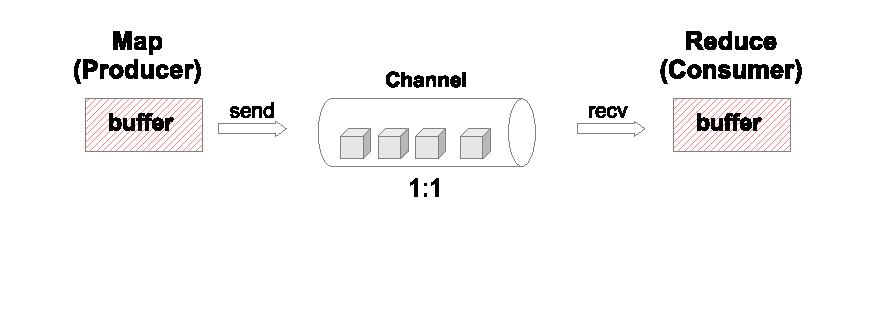
\includegraphics[width=0.4\textwidth]{eps/dmr_channel.eps}
	\caption{Produce-Consume model in SMR}
	\label{fig:dmr:channel}
\end{figure}

%如图所示,这个模型中有两个主要的数据结构:一个map私有buffer pool,其中的每个buffer用于存放发送给对应reduce的数据。一个channel用于mapper和reducer之间数据的传递。
As figure\ref{fig:dmr:channel} shows, there are two major data structures:
a local buffer for each mapper and a one to one
channel used to communicate between mapper and reducer.

Actually, there is a local buffer pool for each mapper.
Each buffer in the pool is used to store key-value 
which is send to a corresponded reducer.
When an intermediate key-value pair is generated by the mapper,
the partition function is used to index the corresponded buffer.
Once the buffer is determined, 
the mapper inserts the key-value into the buffer.
When the buffer threshold is reached,
the map worker will send data into the buffer to the channel by invoking \code{chan\_send}.
Then the reduce worker can read record in the channel by \code{chan\_recv}.
One reduce worker will get key-value from each channel by Round-Robin and 
merge the key-value pairs to the global buffer.

%Figure.\ref{fig:dmr:pc-model} shows producer-conusmer model in our \myds.  
%There is a one to one channel between map worker and reduce worker, 
%avoiding the contention of multiple map workers.
%When the buffer is full, map worker send the buffer to channel, 
%at the same time, 
%reduce worker receive data from channel, and copy it to local buffer.
%on the other hand,
%we use the a special mapping to allow producer and consumer parallelization effectively, 
%without waiting when the queue is full, or malloc and free operations.
%When the local buffer is full,
%it send the data to channel and then use the buffer again.
%That means map no need wait and there is no many malloc and free operations.
%Figure\ref{fig:dmr:pc-model}
%Thus, this parallelization effectively decouples the behavior of proucer and conusmer, and allows them to be overlapped 
%without many malloc and free.
%In Section\ref{} we have present the design of Channel.


%如同Phoenix, 默认情况下,buffer使用hash table来实现,事实上,在我们的模型中,使用array来实现具有更好的性能。下面的章节会详细解释原因。
Defaultly, the buffer is a hash table as Phoenix.
While this technique is more effective for the array buffer
container than the hash buffer. 
We will explain the advantage of array buffer in section 3.2.
MRPhi\cite{lu2013mrphi} is also use producer-consumer model to 
pipeline the map and reduce phases. 
There are partitions queues for each reduce worker.
While we don't use queues, mapping will be used in \myth(section 3.2).







%{\color{gray}
%In the shared-memory model, a region of memory that is shared
%by cooperating processes is established. 
%Processes can then exchange information 
%by reading and writing data to the shared region.
%Shared memory can be faster.
%since in shared-memory systems, system calls are required only to establish shared-memory regions. 
%Once shared memory is established, all accesses are treated
%as routine memory accesses, and no assistance from the kernel is required.
%}
%%SPMC区域的建立
%Interprocess communication using shared memory requires communicating
%processes to establish a region of shared memory. Typically, a shared-memory
%region resides in the address space of the process creating the shared-memory
%segment. Other processes that wish to communicate using this shared-memory
%segment must attach it to their address space. 
%
%%SPMC区域的使用,对应buffer
%To allow producer and consumer processes to run concurrently, we must have
%available a buffer of items that can be filled by the producer and emptied by
%the consumer. This buffer will reside in a region of memory that is shared by
%the producer and consumer processes.(http://bulk.fefe.de/scalability/)



\subsubsection{Buffer Design and Optimize}
Research shows that the organization of MapReduce
intermediate data is a challenge of design a  MapReduce library.
The organization of the Map output is critical to the
performance of many MapReduce applications, 
since the entier body of intermediate data must be
reorganized between the Map and Reduce phase:
Map produces data in the same order as the input,
while Reduce must consume data grouped by key.\cite{mao2010metis}
In a data center this operation is dominated by
the performance of the network, but when running 
on single multicore processor the performance
is dominated by the operations on the data structure
that holds intermediate data.
%已有的工作中,都有哪些buffer,都是如何实现的?

\begin{figure}[!h!t]  
	\centering
	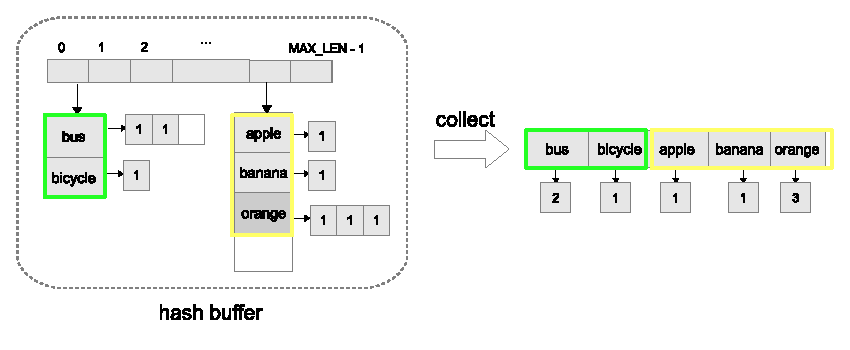
\includegraphics[width=0.5\textwidth]{eps/dmr_hash_buffer.eps}
	\caption{Produce-Consume model in SMR}
	\label{fig:dmr:hash-buffer}
\end{figure}
the element is indexed by the hash value of the key.
Inside each entry of a hash table,

Defaultly, buffer in \myds is a hash table(Figure\ref{fig:dmr:hash-buffer}), 
and each element is a array of pointers to key arrays,
where the fixed is by a default value(256);
\myds stores the key-value pairs in an array sorted by key.
If the hash table have enough entries, 
collisions will be rare and the key arrays will be short,
so that lookup and insert will have cost O(1).
The hash table's O(1) lookups 
make it particularly attractive for workloads with many repeated keys.
{\color{gray}(the reduce operator is immediately applied
	to that pair based on the local container. This process is
	performed using a combiner.)}


Hoverver, our producer-consumer model requires
reduce task is a contiguous block of memory, 
which implies that key-value of hash table should be gathered
before sending to reduce worker.
We address this issue by 
copying values out of the hash tables
at the end of the map phase and 
inserting them into a new contiguous array.
This extra copy is unfortunate and time-consuming.
Furthemore, it also requires frequent allocations and deallocations of memory 
along with the data structure creation and destrcution.

%为了提高效率,避免group阶段产生的开销,我们试图改进buffer的hash实现,它不再采用原来 Phoenix 中的 hash 表的组织方式,而是采用更简单的 array,map worker 产生的 key-value只需追加到 array 中即可,无需排序。

%The buffers are initially sized to a default value and then resized dynamically as needed.
To avoid the time-consuming collection in hash buffer, 
we implement a easy buffer, namely array buffer.
The buffers are initially sized to a default value and 
then reuse the buffer among sub-jobs.
It will indicate that the buffer is empty at the end of a sending, 
but will not free the memory until all map jobs have finished.
Each map thread could store its output 
by appending each key/value pair to array buffer, 
%Map阶段不需要进行排序,而是讲更多排序的工作move给reduce worker
and then as each sub-job is processed in turn,
the data structures and memory spaces 
for the input and intermediate data can be reused across the sub-job boundaries. 
This avoids the costs of expensive memory allocation and deallocation, 
as well as the data structures construction.
This could save the expensive operations 
such as concurrent memory allocations and deallocations,
as well as the building of data structures.
Furthemore, unlike hash buffer, array buffer is a contiguous block of memory,
it not need collection before send the buffer to channel.
For applications that likely have abundant duplicated keys (or values),
such as word\_count, it would be more worthwhile to use array buffer.

% For the array buffer implementation and no combiner in map phase,
% Map just need to . Thus, this technique is more effective
% for array buffer implementation than hash table buffer
% implementation.

%{\color{gray}(A related problem is that eager pipelining moves some of the
%sorting work from the mapper to the reducer.
%Recall that in the
%blocking architecture, map tasks generate sorted output: all the re-
%duce task must do is merge together the pre-sorted map output for
%each partition. In the eager pipelining design, map tasks send out-
%put records in the order in which they are generated, so the reducer
%must perform a full external sort. Because the number of map tasks
%typically far exceeds the number of reduces [4], moving more work
%to the reducer can degrade performance.
%)}




%applications of different buffer as table\ref{diff-buf}
%\begin{table}[]
%\centering
%\caption{My caption}
%\label{diff-buf}
%\begin{tabular}{|l|l|}
%\hline
%\multicolumn{2}{|l|}{\textbf{best buffer of applications}} \\ \hline
%\textbf{application}           & \textbf{buffer}           \\ \hline
%histogram                      & array                     \\ \hline
%word count                     & array                     \\ \hline
%linear regression              & hash                      \\ \hline
%string match                   & hash                      \\ \hline
%pca                            & hash                      \\ \hline
%\end{tabular}
%\end{table}


